%% \subsubsection{General Idea}
\label{subsec:racket-expand}

As described in \secref{sec:intro}, part of the effort of targeting a
new run-time for Racket was making it more portable by separating the
parts that are essential for hosting Racket from the run-time
implementation. \figref{fig:racket-portable} summarizes how different
parts fit together. In the previous versions of Racket, each segment
of the leftmost figure was in C. The first step was to port the
expander from C to Racket, as the Racket expander implements most of
the essential parts for the front-end such as the module system, macro
system, read, expand etc. Aside from being ported from C to Racket,
the expander is also made to elaborate given Racket code into a core
language for the hosting compiler to consume. As we will discuss in
more detail in the remainder of this section, the essential forms of
this language, acting as units of compilation in the run-time, are
called the "linklets", which are lambda-like forms that consume and
produce potentially mutable variables (instead of values).

The way that the expander elaborates a given Racket program is to
produce a bundle of linklets for the different parts of this
program. \figref{fig:racket-expand-example} shows an example where a
Racket module is expanded into such a bundle of linklets. As the
expander strictly separates the expansion and run-time phases, three
linklets are produced for the given source module; one for the
expansion-time (compile-time) and one for the run-time and one for the
literal syntax objects to bridge the two worlds. Linklets can directly
refer to the primitive functions as well. As we will detail in
\secref{subsec:pycket}, they assume rougly 1500 primitive functions
that are implemented in the run-time, such as \emph{vector-ref} and
\emph{+} as it is seen in \figref{fig:racket-expand-example}.

\begin{figure}[h]
  \centering
  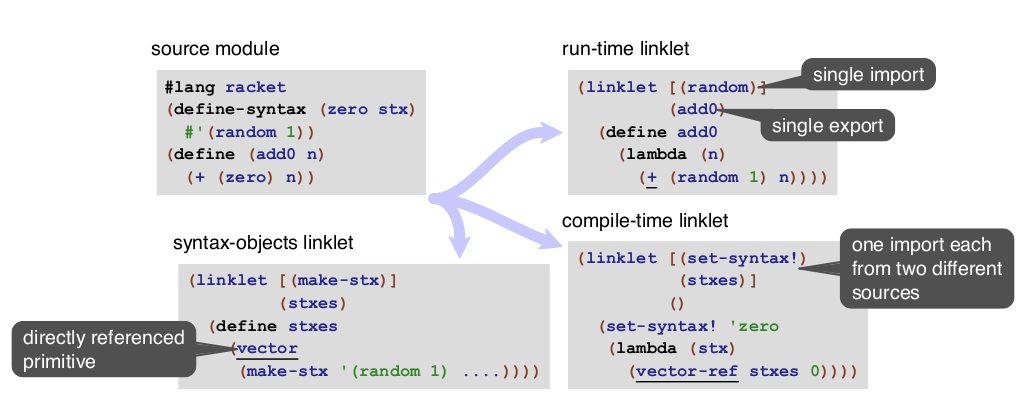
\includegraphics[scale=0.3]{img/racket-expand-example}
  \caption{Expansion of a Racket source module into a linklet
    bundle. Figure used from \cite{racket-on-chez-19}}
  \label{fig:racket-expand-example}
\end{figure}

Using this, just like any other Racket module, when the expander is
given to itself as input, we get an implementation of the expander as
a bundle of linklets that a compiler can consume. Along with the
expander itself, this process (applying the expander) is also used to
export several different functionalities as independent linklets for
the run-time. These linklets are called the
\emph{bootstrapping linklets}. Currently Racket exports four such
linklets: \emph{expander}, \emph{io}, \emph{threads},
\emph{regexp} \footnote{there's also the \emph{schemify} and
  \emph{known} linklets, but they're specifically for Chez Scheme
  integration}. Among them, the \emph{expander} linklet is the key
linklet for making Racket more portable, as it provides the
implementations of essential functionalities such as the module
system, macro system, read, eval etc.

A hosting compiler that implements a thin API layer to process
linklets (the \emph{linklets} layer in \figref{fig:racket-portable})
can then consume these bootstrapping linklets to load the essential
functionalities into its run-time, for example loading the expander
linklet to read, expand and evaluate any given Racket code. That API
is usually accommodated with an adapter layer in the run-time. For
example in Chez Scheme, the \emph{schemify} layer in the rightmost
figure of the \figref{fig:racket-portable} converts the produced
linklets into Chez Scheme lambda forms. We will discuss the
implementation and use of this API in more detail in
\secref{subsec:pycket}.
